\begin{frame}{Black Box Modelling with Neural Nets}
    Previous work: Damsk{\"a}gg et al., 2019\footcite[]{WaveNetVA}
    \vspace{1ex}
    \begin{itemize}
        \itemsep0.5em
        \item Uses a WaveNet-style, ``Temporal Convolutional Network''
        \item Used to model distortion pedal circuits
        \item Also used to model tube amp distortion\footcite[]{damskgg2018deep}
        \item Disadvantage: computationally expensive
    \end{itemize}
\end{frame}

\begin{frame}{Temporal Convolutional Networks}
    Keith Bloemer: Smart Guitar Amp\footnote{\url{https://github.com/keyth72/SmartGuitarAmp}}
    \begin{figure}
        \centering
        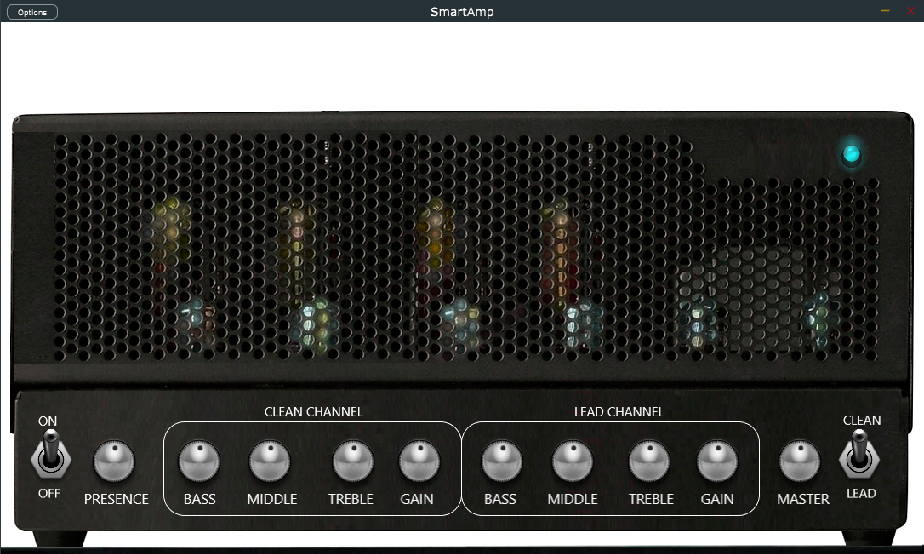
\includegraphics[height=2.25in]{Figures/SmartAmp.png}
    \end{figure}
\end{frame}

\begin{frame}{Temporal Convolutional Networks}
    Christian Steinmetz: Randomized Overdrive Neural Networks\footnote{\url{https://github.com/csteinmetz1/ronn}}
    \begin{figure}
        \centering
        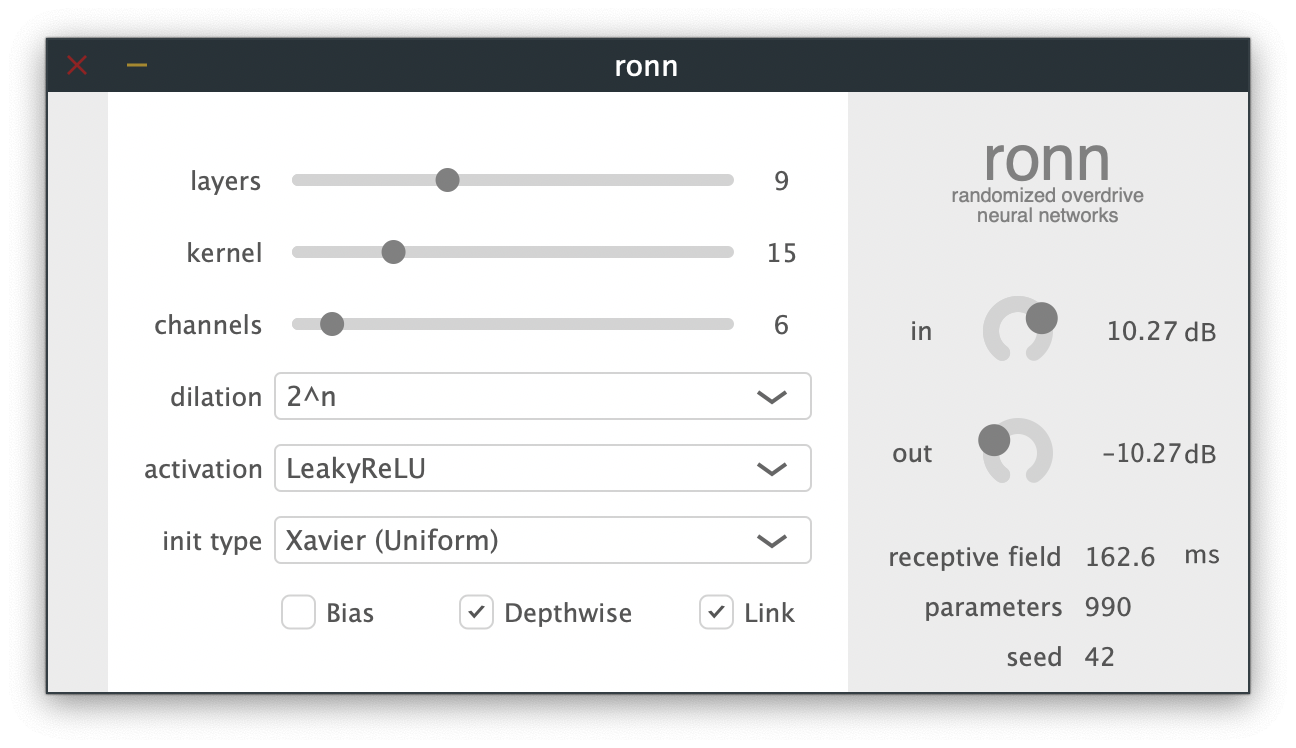
\includegraphics[height=2.25in]{Figures/ronn-vst-ui.png}
    \end{figure}
\end{frame}

% \begin{frame}{Temporal Convolutional Networks}
%     Neural DSP (probably\dots)
%     \begin{figure}
%         \centering
%         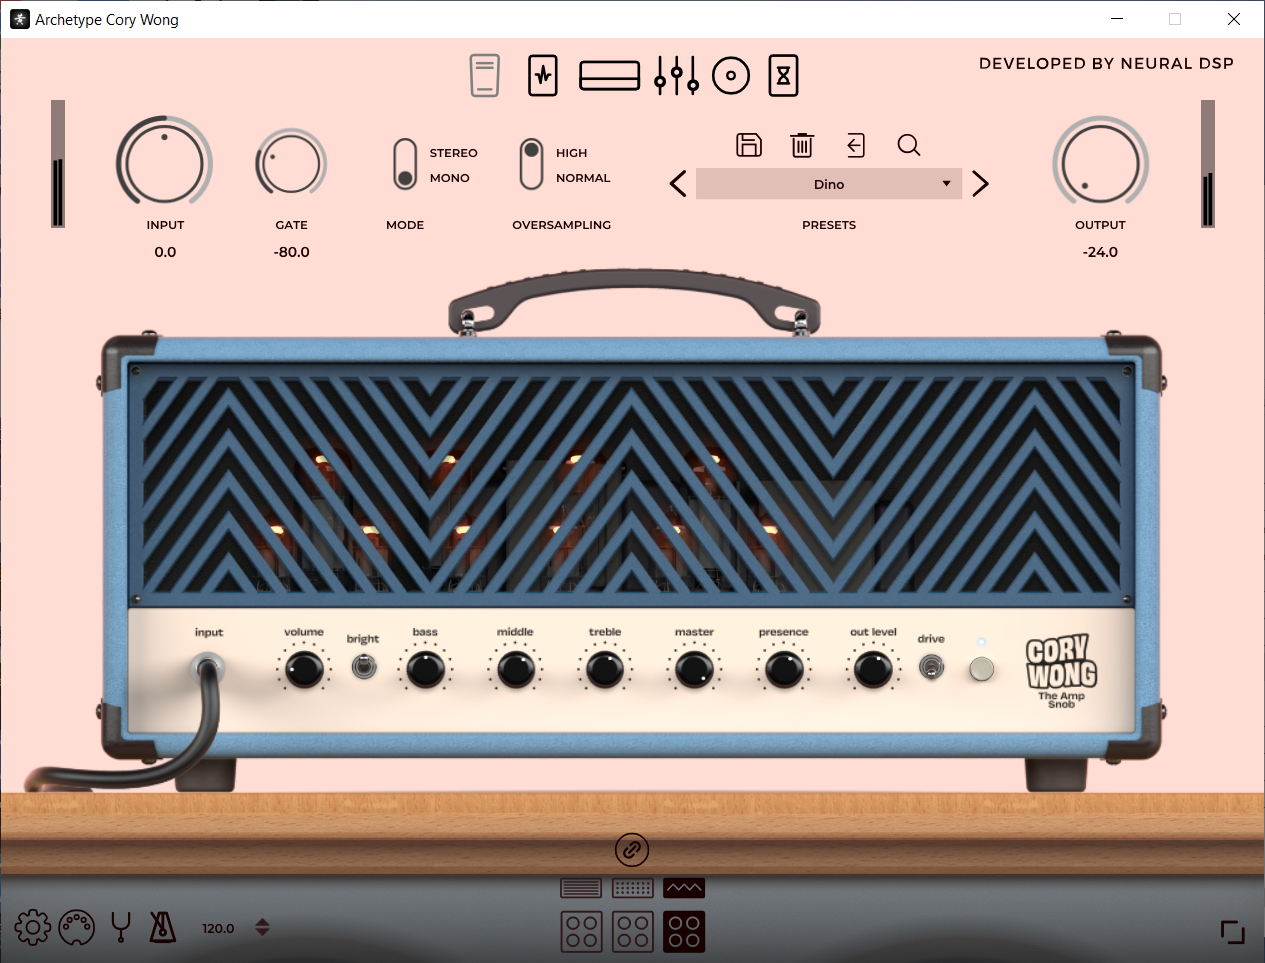
\includegraphics[height=2.5in]{Figures/neuraldsp.png}
%     \end{figure}
% \end{frame}

\begin{frame}{Black Box Modelling with Neural Nets}
    Previous work: Parker et al., 2019\footcite[]{NLML}
    \vspace{1ex}
    \begin{itemize}
        \itemsep0.5em
        \item Uses a deep, fully-connected ``State Transition Network''
        \item Approximates a state-space solution for nonlinear distortion and filter circuits
        \item Effectively a ``grey-box'' model
    \end{itemize}
\end{frame}

\begin{frame}{State Transition Networks}
    Native Instruments: Guitar Rig 6 Pro\footnote{\url{https://blog.native-instruments.com/the-making-of-icm/}}
    \begin{figure}
        \centering
        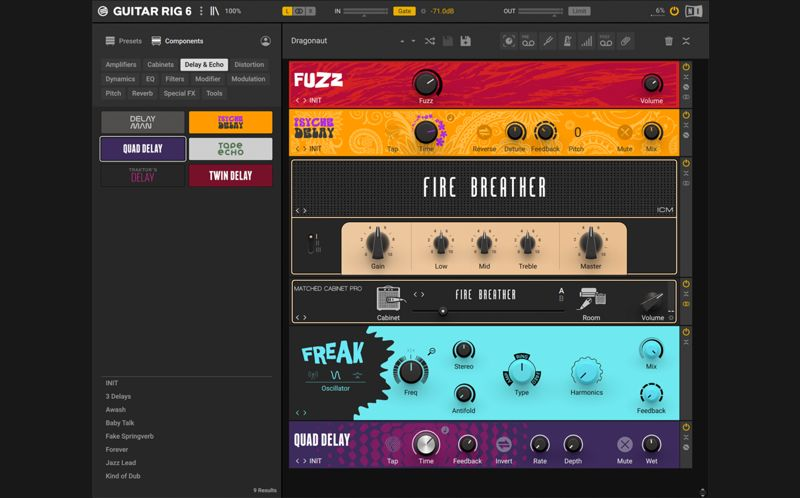
\includegraphics[height=2.25in]{Figures/GuitarRig6.jpg}
    \end{figure}
\end{frame}

\begin{frame}{Black Box Modelling with Neural Nets}
    Previous work: Wright et al., 2019\footcite[]{VArnn}
    \vspace{1ex}
    \begin{itemize}
        \itemsep0.5em
        \item Uses a single layer recurrent neural network
        \item Used to model guitar distortion circuits
        \item Can also be used to model time-varying circuits\footcite[]{RNNtime}
    \end{itemize}
\end{frame}
